\documentclass{article}[18pt]
\usepackage{../../../../format}
\lhead{AS Level Physics - Mechanics and Materials}

\begin{document}
\begin{center}
\underline{\huge Force, Energy and Momentum}
\end{center}
\section{Scalars and Vectors}
\textbf{Scalar} - Magnitude\\
\textbf{Vector} - Magnitude and Direction
\section{Moments}
\subsection{Moment}
$$\text{Force}\times \text{Perpendicular distance from the point to the line of action of the force}$$
\subsection{Couple}
$$\text{A pair of equal and opposite coplanar forces}$$
\subsection{Moment of a couple}
$$\text{Force}\times\text{Perpendicular distance between the lines of action of the forces}$$
\subsection{Principle of moments}
\begin{center}
For an object in equilibrium, \textbf{Clockwise Moments=Anticlockwise Moments}
\end{center}
\section{Graphs with respect to time}
\begin{tabularx}{\textwidth}{|X|X|X|}
\hline
\textbf{Type of Graph}&\textbf{Gradient}&\textbf{Area Under Graph}\\
\hline
Distance Time&Velocity&-\\
\hline
Velocity time&Acceleration&Displacement\\
\hline
Acceleration time&-&Change in velocity\\
\hline
\end{tabularx}
\section{Projectile motion}
For a falling object with no air resistance there is no horizontal acceleration or deceleration 
\subsection{Terminal Velocity}

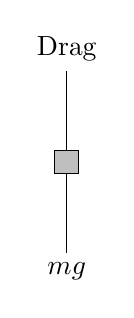
\begin{tikzpicture}[
    force/.style={>=latex,draw=blue,fill=blue},
    m/.style={rectangle,draw=black,fill=lightgray,minimum size=0.3cm,thin},
]
    \node[m] (m) {};
    {[force,->]
        \draw (m.north) -- ++(0,1) node[above] {Drag};
        \draw (m.south) -- ++(0,-1) node[below] {$mg$};
    }
\end{tikzpicture}\\
As an object accelerates speed increases so drag increases, when \textbf{Drag=mg} the object has reached \textbf{terminal velocity} meaning that it now travels at a \textbf{constant velocity}
\subsection{The effect of air resistance}
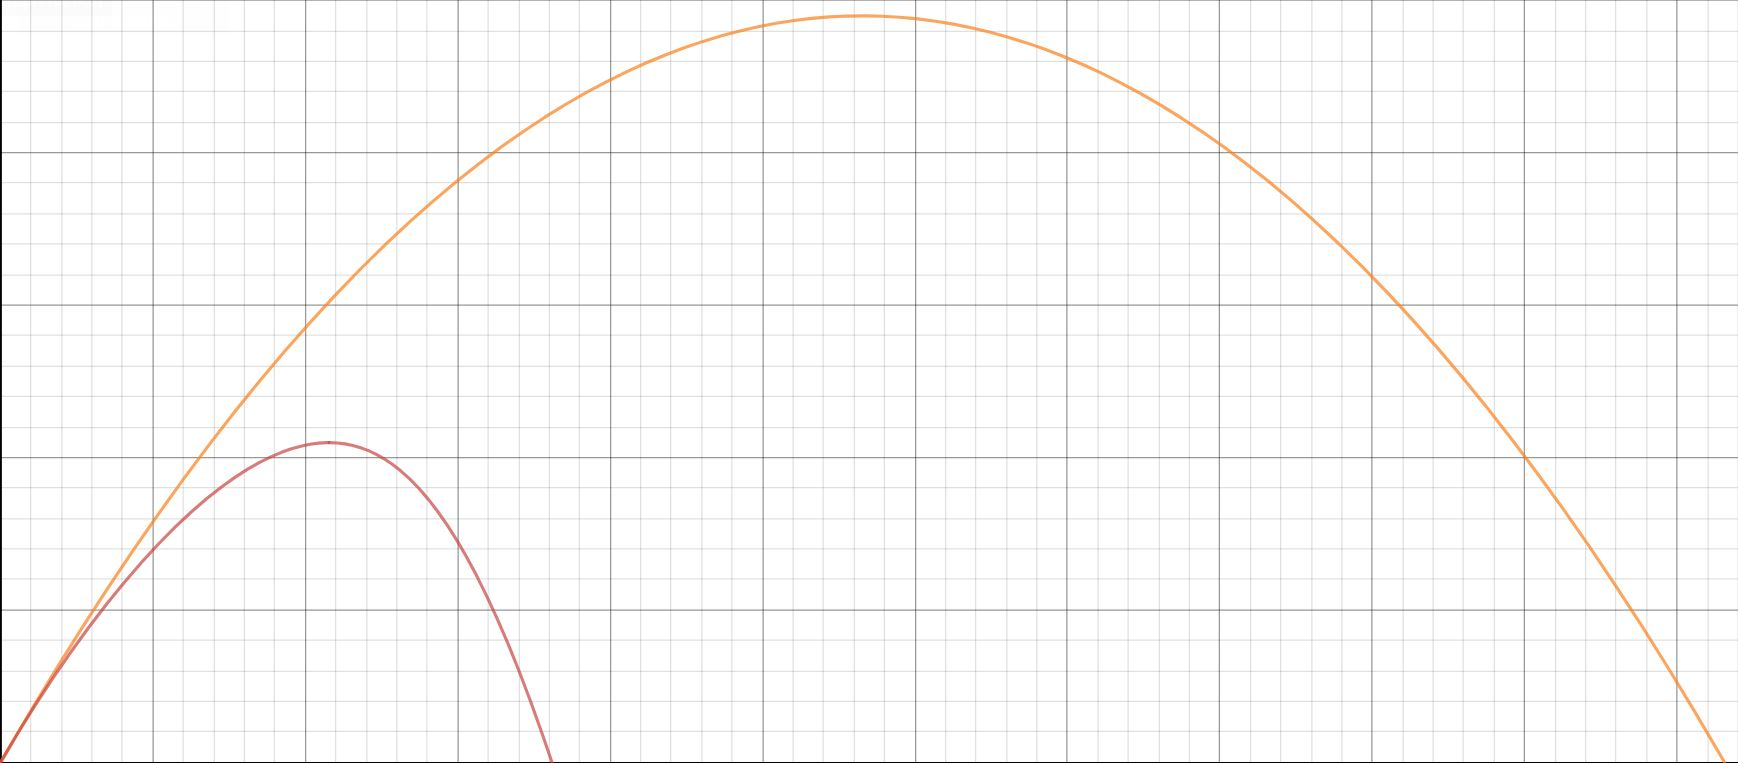
\includegraphics[scale=0.25]{Air_Resistance.JPG}\\
\textcolor{orange}{No Air Resistance}\\
\textcolor{red}{Air resistance
\begin{itemize}
\item Steeper descent
\item Peak Further Left
\item Smaller Range
\end{itemize}}
\subsubsection{Factors that affect air resistance}
\begin{itemize}
\item Surface area
\item Air Pressure/Density
\item Speed
\item Roughness of shape
\end{itemize}
\section{Newton's laws of motion}
\textbf{First Law} - Objects either stay at rest or move with a constant velocity unless acted on by a resultant force\\
\textbf{Second law} - For an object with constant mass its acceleration will be directly proportional to the resultant force $F=ma$\\
\textbf{Third law} - Every action has an equal and opposite reaction
\section{Momentum}
$\text{Momentum=Mass}\times\text{Velocity}$\\
In a collision \textbf{Momentum is conserved}\\
\textbf{Impulse}=Change in momentum\\
The area under a force time graph is the impulse\\
\textbf{Elastic collision} - A collision with no loss of kinetic energy\\
\textbf{Inelastic collision} - A collision with a loss of kinetic energy
\section{Work, energy and power}
Rate of doing work=Rate of energy transfer\\
The area under a force displacement graph is the \textbf{work done}
\section{Conservation of energy}
\textbf{Principle of conservation of energy} - In an isolated system the total energy remains constant


\end{document}
